\documentclass[dp]{FEIstyle}

% Author of the thesis
\FEIauthor{Bc. Jakub Hubáček}

% Evidence number
\FEIregNr{FEI-104378-115323}

% Title
\FEItitle{Mobilná aplikácia na ovládanie výrobnej linky s využitím jedinečného identifikátora}
\FEItitleEn{Mobile application for controlling a production line using a unique identifier}

% Date
\FEIdate{15}{5}{2026}

% Keywords
\FEIkeywords{Ovládanie výrobnej linky, mobilná aplikácia, jedinečný identifikátor, AI asistent}
\FEIkeywordsEn{Production line control, mobile application, unique identifier, AI assistant}

% Further details
\FEIstudyProgramme{Aplikovaná mechatronika a elektromobilita}
\FEIstudyProgrammeEn{Applied Mechatronics and Electromobility}
\FEIstudyField{Kybernetika}
\FEIstudyFieldEn{Cybernetics}
\FEItrainingWorkplace{Ústav automobilovej mechatroniky (FEI)}
\FEItrainingWorkplaceEn{Institute of Automotive Mechatronics (FEI)}

% Supervisor
\FEIsupervisor{Ing. Lukáš Beňo PhD.}

% Consultant
% -- if there is none, comment out the next line
% \FEIconsultant{tituly Meno Priezvisko, tituly}

% Glossaries -- terms and abbreviations.
% If you use automatic glossaries,
% uncomment the next line.
\FEIglossaries{includes/glossary}

% Bibliography database file
\bibliography{includes/bibliography.bib}

\begin{document}

%%%%%%%%%%%%%%%%%%
%%              %%
%% FRONT MATTER %%
%%              %%
%%%%%%%%%%%%%%%%%%
\frontmatter

\FEIpdfInfo
\FEIcover
\FEItitlePage
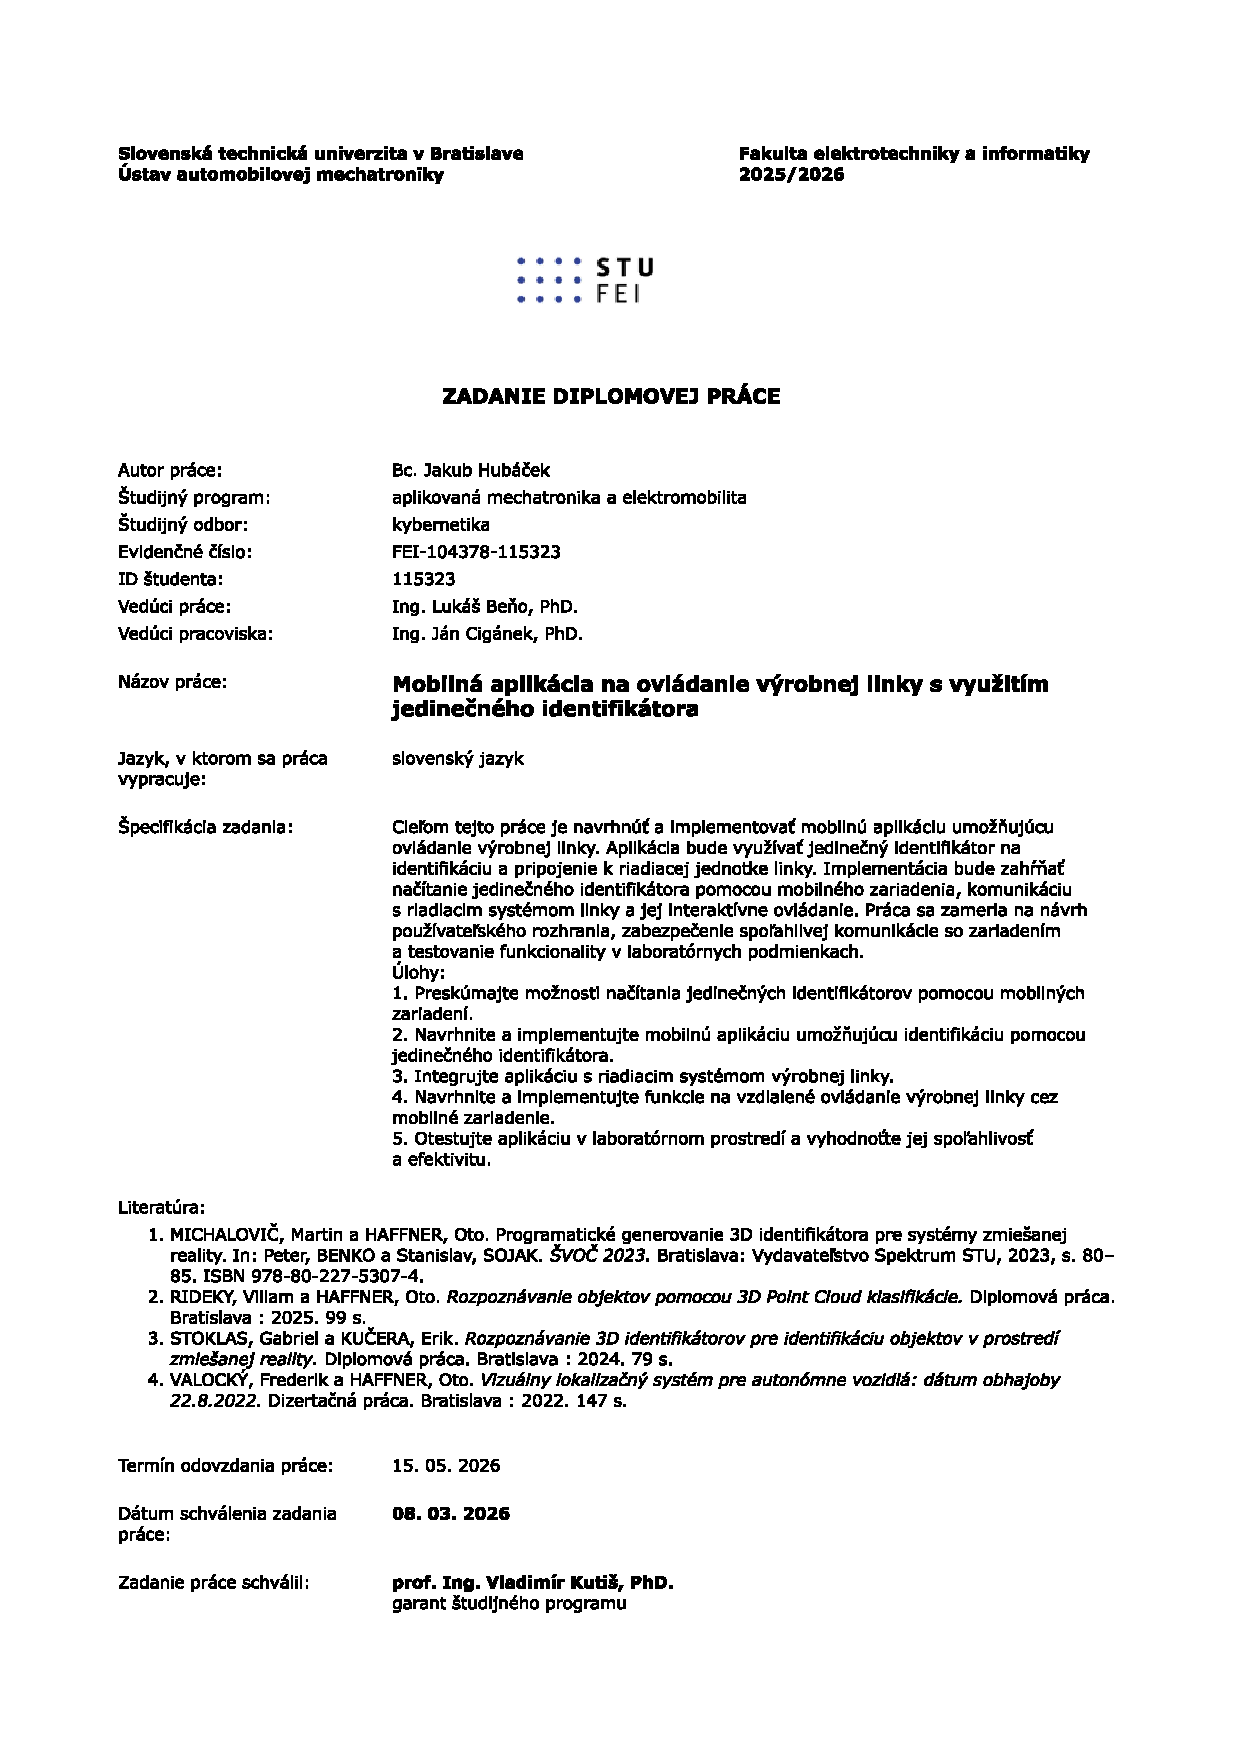
\includepdf[pages=-]{img/zadanie.pdf}
\FEIthanks{includes/thanks}
\FEIabstract{includes/abstract}
\FEIabstractEn{includes/abstractEN}
\FEIcontent
\FEIlistOfFiguresAndTables

%% List of units and abbreviations
%%
%% Choose the method of typesetting the list of
%% units and abbreviations.
%% Uncomment only one of the two lines below!

%% METHOD 1:
%% ---------
%% Automatically generated and sorted list of
%% abbreviations with hyperlinks from the text.
%% Edit includes/glossary.tex.
\FEIlistOfGlossaries
%% METHOD 2:
%% ---------
%% Manual list -- must be manually filled and sorted,
%% does not make hyperlinks from the text.
%% Edit includes/manual_glossary.tex.
%\FEImanualListOfGlossaries{includes/manual_glossary}

%% Lists of algorithms and listings
%\FEIlistOfAlgorithms
\FEIlistOfListings

%%%%%%%%%%%%%%%%%
%%             %%
%% MAIN MATTER %%
%%             %%
%%%%%%%%%%%%%%%%%
\mainmatter
\setcounter{page}{1}

\FEIintroduction{includes/introduction}
\FEIcore{includes/core}
\FEIconclusion{includes/conclusion}

%% Uncomment only if the document is writen in english
%\FEIresume{includes/resume}

%%%%%%%%%%%%%%%%%%
%%              %%
%% Bibliography %%
%%              %%
%%%%%%%%%%%%%%%%%%
\FEIbibliography
%% AI Declaration
\FEIaiDeclaration{includes/ai_declaration}

%%%%%%%%%%%%%%%%%%
%%              %%
%% BACK MATTER  %%
%%              %%
%%%%%%%%%%%%%%%%%%
\backmatter

%% Attachment A
\FEIappendix{Súborová štruktúra\label{att:filesystem}}{includes/attachmentA}

%% Attachment B
\FEIappendix{Prílohy k testovaniu\label{att:testing}}{includes/attachmentB}

%% Attachment C
\FEIappendix{Návod na spustenie\label{att:launch}}{includes/attachmentC}

%% Attachement D
\FEIappendix{Opis funkcionalít aplikácie\label{att:functionality}}{includes/attachmentD}


\end{document}
